\documentclass[paper=a4, fontsize=11pt]{scrartcl} 

\usepackage[T1]{fontenc} 
\usepackage[english]{babel}
\usepackage{amsmath,amsfonts,amsthm}

\usepackage{lipsum}

\usepackage{graphicx}
\usepackage{float}
  \floatplacement{figure}{H}
  \floatplacement{table}{H}
  
\usepackage{sectsty} 
\allsectionsfont{\centering \normalfont\scshape} 

\usepackage{fancyhdr} % Custom headers and footers
\pagestyle{fancyplain} % Makes all pages in the document conform to the custom headers and footers
\fancyhead{} % No page header - if you want one, create it in the same way as the footers below
\fancyfoot[L]{} % Empty left footer
\fancyfoot[C]{} % Empty center footer
\fancyfoot[R]{\thepage} % Page numbering for right footer
\renewcommand{\headrulewidth}{0pt} % Remove header underlines
\renewcommand{\footrulewidth}{0pt} % Remove footer underlines
\setlength{\headheight}{13.6pt} % Customize the height of the header

\usepackage[labelformat=empty]{caption}
\usepackage{color}
\usepackage{listings}
\lstset{ %
language=bash,                % choose the language of the code
basicstyle=\footnotesize,       % the size of the fonts that are used for the code
numbers=left,                   % where to put the line-numbers
numberstyle=\footnotesize,      % the size of the fonts that are used for the line-numbers
stepnumber=1,                   % the step between two line-numbers. If it is 1 each line will be numbered
numbersep=5pt,                  % how far the line-numbers are from the code
backgroundcolor=\color{white},  % choose the background color. You must add \usepackage{color}
showspaces=false,               % show spaces adding particular underscores
showstringspaces=false,         % underline spaces within strings
showtabs=false,                 % show tabs within strings adding particular underscores
frame=single,           % adds a frame around the code
tabsize=2,          % sets default tabsize to 2 spaces
captionpos=b,           % sets the caption-position to bottom
breaklines=true,        % sets automatic line breaking
breakatwhitespace=false,    % sets if automatic breaks should only happen at whitespace
escapeinside={\%*}{*)}          % if you want to add a comment within your code
}



\numberwithin{equation}{section} % Number equations within sections (i.e. 1.1, 1.2, 2.1, 2.2 instead of 1, 2, 3, 4)
\numberwithin{figure}{section} % Number figures within sections (i.e. 1.1, 1.2, 2.1, 2.2 instead of 1, 2, 3, 4)
\numberwithin{table}{section} % Number tables within sections (i.e. 1.1, 1.2, 2.1, 2.2 instead of 1, 2, 3, 4)

\setlength\parindent{0pt} % Removes all indentation from paragraphs - comment this line for an assignment with lots of text

%----------------------------------------------------------------------------------------
%	TITLE SECTION
%----------------------------------------------------------------------------------------

\newcommand{\horrule}[1]{\rule{\linewidth}{#1}} % Create horizontal rule command with 1 argument of height

\title{	
\normalfont \normalsize 
\textsc{Computational Science - ITB} \\ [25pt] % Your university, school and/or department name(s)
\horrule{0.5pt} \\[0.4cm] % Thin top horizontal rule
\small  Pengenalan Sains Komputasi - Fitting data\\ % The assignment title
%\horrule{2pt} \\[0.5cm] % Thick bottom horizontal rule
}

\author{\small{Ridlo W. Wibowo || 20912009}} % Your name

\date{\normalsize\today} % Today's date or a custom date

\begin{document}

\maketitle % Print the title

\large \textbf{Problem.}\\
Fitting 2 set data yang ada dengan menggunakan software atau tools fitting dari bahasa pemrograman anda.\\

\large \textbf{Documentation.}\\
Data yang dipilih dari sumber:
\begin{enumerate}
\item NorrisEM.txt (untuk coba-coba terlebih dahulu)
\item FilipEM.txt
\item Gauss1.txt
\end{enumerate}
Software yang digunakan adalah \texttt{gnuplot} (OS: Ubuntu).\\

Setelah dilakukan perbaikan format data (karena tidak bisa dibaca oleh \texttt{gnuplot -- ubuntu}), maka proses fitting dilakukan dengan cara sederhana, yaitu menentukan fungsi fitting yang ingin kita gunakan lalu menggunakan fungsi \texttt{fit} yang ada di dalam gnuplot (lihat dokumentasi gnuplot). Fungsi ini adalah implementasi algoritma \textit{Levenberg-Marquardt} untuk nonlinear least-squares (NLLS) pada \texttt{gnuplot}.\\

\begin{enumerate}
\item \textbf{NorrisEM.txt}\\
Kita ingin melakukan fitting data ini menggunakan fungsi linier (garis lurus) dengan persamaan:
\begin{equation}
y = a + bx
\end{equation}
dengan fungsi \textit{fit} yang ada pada gnuplot kita ingin menentukan konstanta $a$ dan $b$ yang menjadikan fungsi di atas dapat menggambarkan data yang ada, atau sering disebut regresi linier.\\

%\newpage
Langkah-langkahnya, pertama kita buat file input untuk gnuplot agar pengerjaan lebih mudah (\textit{norris.in}):
\lstset{frameround=fttt}
\begin{lstlisting} %%[frame=trBL]
set term png
set output "norris.png"
set xlabel "x"
set ylabel "y = f(x)"
f(x) = a + b*x
fit f(x) "Norris.txt" using 1:2 via a,b
plot "Norris.txt" u 1:2 title "data", f(x) title "fitting function"
\end{lstlisting}
kemudian dapat dijalankan dengan perintah sederhana (di ubuntu):
\lstset{numbers=none}
\begin{lstlisting}
$ gnuplot < norris.in
\end{lstlisting}
\texttt{gnuplot} akan melakukan iterasi dan menghasilkan fitting terbaik dengan toleransi tertentu, dalam kasus ini:
\begin{small}
\begin{verbatim}
After 5 iterations the fit converged.
final sum of squares of residuals : 26.5049
rel. change during last iteration : -7.49057e-06

degrees of freedom    (FIT_NDF)                        : 34
rms of residuals      (FIT_STDFIT) = sqrt(WSSR/ndf)    : 0.882925
variance of residuals (reduced chisquare) = WSSR/ndf   : 0.779556

Final set of parameters            Asymptotic Standard Error
=======================            ==========================

a               = 0.264389         +/- 0.2322       (87.84%)
b               = 0.997881         +/- 0.000428     (0.04289%)


correlation matrix of the fit parameters:

               a      b      
a               1.000 
b              -0.774  1.000 
\end{verbatim}
\end{small}
dan menggunakan perintah di atas kita juga akan peroleh plot data dan fungsi hasil fittingnya:
\begin{figure}
	\centering
	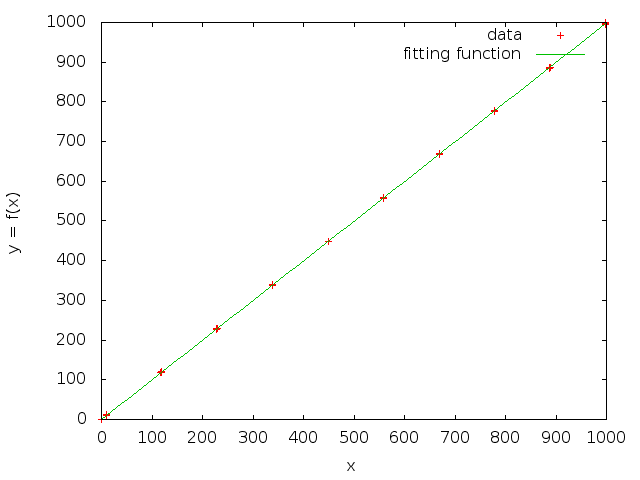
\includegraphics[width=0.8\textwidth]
		{norris.png}
	\caption{\textit{NorrisEM.txt dan fungsi fittingnya}.}
\end{figure}

diperoleh fungsi fitting:
\begin{equation}
y = 0.264389 + 0.997881x
\end{equation}\\

\item \textbf{FilipEM.txt}\\
Kita ingin melakukan fitting data ini menggunakan fungsi polinom dengan persamaan:
\begin{equation}
y = a_{0} + a_{1}x + a_{2}x^{2} + a_{3}x^{3} + a_{4}x^{4} + a_{5}x^{5} + a_{6}x^{6} + a_{7}x^{7} + a_{8}x^{8} + a_{9}x^{9} + a_{10}x^{10}
\end{equation}
dengan fungsi \textit{fit} yang ada pada gnuplot kita ingin menentukan 11 konstanta pada persamaan di atas.
Langkahnya sama seperti sebelumnya, pertama kita buat file input untuk gnuplot (\textit{filip.in}):
\lstset{frameround=fttt}
\begin{lstlisting} %%[frame=trBL]
set term png
set output "filip.png"
set xlabel "x"
set ylabel "y = f(x)"
f(x) = a0 + a1*x + a2*x**2 + a3*x**3 + a4*x**4 + a5*x**5 + a6*x**6 + a7*x**7 + a8*x**8 + a9*x**9 + a10*x**10
fit f(x) "Filip.txt" using 1:2 via a0,a1,a2,a3,a4,a5,a6,a7,a8,a9,a10
plot "Filip.txt" using 1:2 title "data", f(x) title "fitting polynomial"
\end{lstlisting}
kemudian jalankan \texttt{gnuplot}:
\lstset{numbers=none}
\begin{lstlisting}
$ gnuplot < filip.in
\end{lstlisting}

Hasil:
\begin{small}
\begin{verbatim}
After 16 iterations the fit converged.
final sum of squares of residuals : 2.88774
rel. change during last iteration : -9.30383e-06

degrees of freedom    (FIT_NDF)                        : 71
rms of residuals      (FIT_STDFIT) = sqrt(WSSR/ndf)    : 0.201674
variance of residuals (reduced chisquare) = WSSR/ndf   : 0.0406724

Final set of parameters            Asymptotic Standard Error
=======================            ==========================

a0              = 2.00527e+07      +/- 2.549e+08    (1271%)
a1              = 1.0012e+09       +/- 2.59e+09     (258.7%)
a2              = -9.27085e+09     +/- 1.495e+10    (161.3%)
a3              = 3.31814e+10      +/- 5.965e+10    (179.8%)
a4              = -5.90527e+10     +/- 1.597e+11    (270.4%)
a5              = 4.47287e+10      +/- 2.865e+11    (640.6%)
a6              = 1.95601e+10      +/- 3.478e+11    (1778%)
a7              = -7.31835e+10     +/- 2.831e+11    (386.9%)
a8              = 6.65244e+10      +/- 1.486e+11    (223.4%)
a9              = -2.83802e+10     +/- 4.561e+10    (160.7%)
a10             = 4.87144e+09      +/- 6.229e+09    (127.9%)


correlation matrix of the fit parameters:

               a0     a1     a2     a3     a4     a5     a6     a7     a8     a9     a10    
a0              1.000 
a1             -0.887  1.000 
a2              0.550 -0.872  1.000 
a3             -0.212  0.634 -0.930  1.000 
a4             -0.015 -0.435  0.816 -0.970  1.000 
a5              0.160  0.290 -0.712  0.917 -0.986  1.000 
a6             -0.255 -0.184  0.624 -0.861  0.957 -0.992  1.000 
a7              0.319  0.103 -0.549  0.807 -0.923  0.973 -0.995  1.000 
a8             -0.363 -0.039  0.485 -0.756  0.886 -0.949  0.981 -0.996  1.000 
a9              0.394 -0.012 -0.428  0.707 -0.848  0.922 -0.963  0.986 -0.997  1.000 
a10            -0.415  0.054  0.377 -0.661  0.811 -0.893  0.941 -0.971  0.988 -0.997  1.000 
\end{verbatim}
\end{small}

\newpage
plot data dan fungsi hasil fittingnya:
\begin{figure}
	\centering
	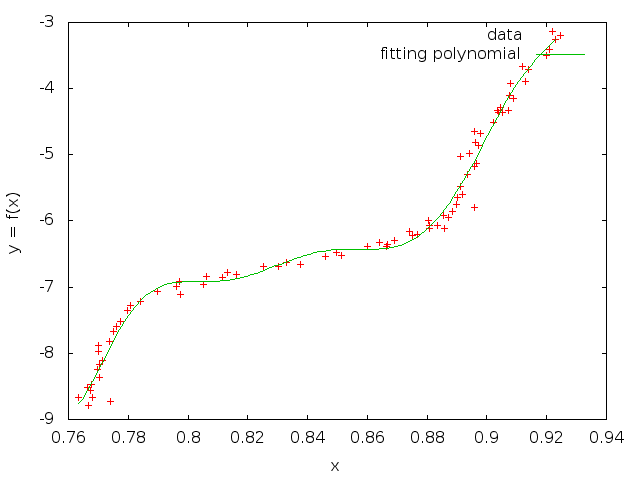
\includegraphics[width=0.8\textwidth]
		{filip.png}
	\caption{\textit{FilipEM.txt dan fungsi fittingnya}.}
\end{figure}


\item \textbf{Gauss1EM.txt}\\
Kita ingin melakukan fitting data ini menggunakan fungsi gauss dengan persamaan:
\begin{equation}
y = f(x) = a_{0}e^{-a_{1}x} + a_{2}e^{\frac{-(x-a_{3})^{2}}{a_{4}^{2}}} + a_{5}e^{\frac{-(x-a_{6})^{2}}{a_{7}^{2}}}
\end{equation}
dengan fungsi \textit{fit} yang ada pada gnuplot kita ingin menentukan 7 konstanta pada persamaan di atas. 

Data yang ada ternyata harus ditukar kolomnya apabila kita ingin melakukan fitting suatu funngsi.

Langkahnya hampir sama seperti sebelumnya, namun untuk kasus ini setelah dicoba ternyata tidak akan konvergen apabila kita tidak memasukkan tebakan awal nilai konstanta yang cukup dekat dengan data yang ada. Setelah memperkirakan berapa nilai untuk tebakan awal sesuai data yang ada, kita dapat memasukkannya ke dalam file input untuk gnuplot (\textit{gauss.in}) sehingga menjadi seperti berikut ini:

%\newpage
\lstset{frameround=fttt}
\begin{lstlisting}
set term png
set output "gauss.png"
set xlabel "x"
set ylabel "y = f(x)"
a0 = 80
a1 = 0.01
a2 = 100
a3 = 50
a4 = 15
a5 = 70
a6 = 170
a7 = 18
f(x) = a0*exp(-a1*x) + a2*exp((-(x-a3)**2)/(a4**2)) + a5*exp((-(x-a6)**2)/(a7**2))
fit f(x) "Gauss.txt" using 2:1 via a0,a1,a2,a3,a4,a5,a6,a7
plot "Gauss.txt" using 2:1 title "data", f(x) title "fitting function"
\end{lstlisting}
kemudian jalankan \texttt{gnuplot}:

\lstset{numbers=none}
\begin{lstlisting}
$ gnuplot < gauss.in
\end{lstlisting}

Hasil:
\begin{small}
\begin{verbatim}
After 8 iterations the fit converged.
final sum of squares of residuals : 1315.82
rel. change during last iteration : -2.38286e-10

degrees of freedom    (FIT_NDF)                        : 242
rms of residuals      (FIT_STDFIT) = sqrt(WSSR/ndf)    : 2.3318
variance of residuals (reduced chisquare) = WSSR/ndf   : 5.43728

Final set of parameters            Asymptotic Standard Error
=======================            ==========================

a0              = 98.778           +/- 0.5754       (0.5825%)
a1              = 0.0104972        +/- 0.0001142    (1.088%)
a2              = 100.49           +/- 0.5883       (0.5855%)
a3              = 67.4811          +/- 0.1046       (0.155%)
a4              = 23.1297          +/- 0.1745       (0.7544%)
a5              = 71.9943          +/- 0.626        (0.8696%)
a6              = 178.998          +/- 0.1244       (0.06948%)
a7              = 18.3893          +/- 0.2014       (1.095%)


correlation matrix of the fit parameters:

               a0     a1     a2     a3     a4     a5     a6     a7     
a0              1.000 
a1              0.494  1.000 
a2             -0.084  0.328  1.000 
a3              0.281  0.237  0.026  1.000 
a4             -0.271  0.321 -0.175 -0.019  1.000 
a5              0.076  0.301  0.122  0.056  0.138  1.000 
a6              0.010 -0.055 -0.030 -0.005 -0.039 -0.013  1.000 
a7              0.107  0.470  0.195  0.084  0.222 -0.324 -0.038  1.000 
\end{verbatim}
\end{small}

plot data dan fungsi hasil fittingnya:
\begin{figure}
	\centering
	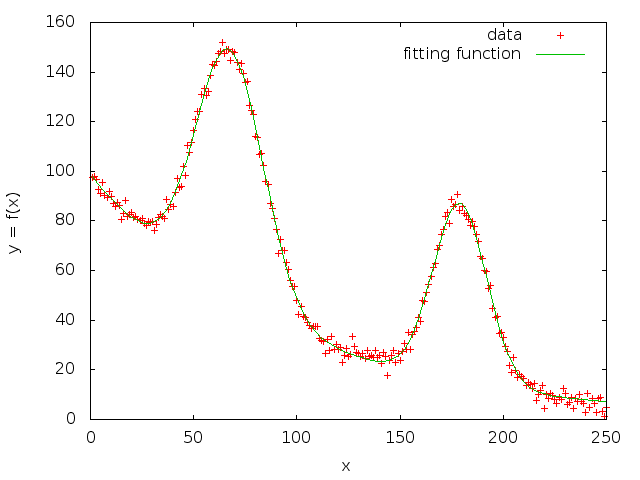
\includegraphics[width=0.8\textwidth]
		{gauss.png}
	\caption{\textit{Gauss1EM.txt dan fungsi fittingnya}.}
\end{figure}

\vspace{8cm}
\begin{center}
== *** ==
\end{center}
\end{enumerate}




\end{document}














